% !TeX spellcheck = en_US
%%%%%%%%%%%%%%%%%%%%%%% file template.tex %%%%%%%%%%%%%%%%%%%%%%%%%
%
% This is a general template file for the LaTeX package SVJour3
% for Springer journals.          Springer Heidelberg 2010/09/16
%
% Copy it to a new file with a new name and use it as the basis
% for your article. Delete % signs as needed.
%
% This template includes a few options for different layouts and
% content for various journals. Please consult a previous issue of
% your journal as needed.
%
%%%%%%%%%%%%%%%%%%%%%%%%%%%%%%%%%%%%%%%%%%%%%%%%%%%%%%%%%%%%%%%%%%%
%
% First comes an example EPS file -- just ignore it and
% proceed on the \documentclass line
% your LaTeX will extract the file if required
\begin{filecontents*}{example.eps}
	%!PS-Adobe-3.0 EPSF-3.0
	%%BoundingBox: 19 19 221 221
	%%CreationDate: Mon Sep 29 1997
	%%Creator: programmed by hand (JK)
	%%EndComments
	gsave
	newpath
	20 20 moveto
	20 220 lineto
	220 220 lineto
	220 20 lineto
	closepath
	2 setlinewidth
	gsave
	.4 setgray fill
	grestore
	stroke
	grestore
\end{filecontents*}
%
\RequirePackage{fix-cm}
%
%\documentclass{svjour3}                     % onecolumn (standard format)
%\documentclass[smallcondensed]{svjour3}     % onecolumn (ditto)
\documentclass[smallextended]{svjour3}       % onecolumn (second format)
%\documentclass[twocolumn]{svjour3}          % twocolumn
%
\smartqed  % flush right qed marks, e.g. at end of proof
%
\usepackage{graphicx}
\usepackage{lipsum}
%\usepackage{sectsty}
\usepackage{pdfpages}
\usepackage{float}
\usepackage{caption}  % subfigures
\usepackage{subcaption} % subfigures
\usepackage{nicefrac}
\usepackage{url}
\usepackage{booktabs}
%
% \usepackage{mathptmx}      % use Times fonts if available on your TeX system
%
% insert here the call for the packages your document requires
%\usepackage{latexsym}
% etc.
%
% please place your own definitions here and don't use \def but
% \newcommand{}{}
%
% Insert the name of "your journal" with
\journalname{Empirical Software Engieenering}

\begin{document}
	
	\title{
		The Perception of Practitioners of Continuous Integration on Its Impact on the Delivery Time of Merged Pull Requests
	}
	%\subtitle{Do you have a subtitle?\\ If so, write it here}
	
	%\titlerunning{Short form of title}        % if too long for running head
	
	\author{João Helis Bernardo         \and
		Daniel Alencar da Costa \and 
		Uirá Kulesza \and 
		Christoph Treude \and 
	}
	
	%\authorrunning{Short form of author list} % if too long for running head
	
	\institute{João Helis Bernardo \at
		Federal Institute of Rio Grande do Norte (IFRN) \\
		%              Tel.: +123-45-678910\\
		%              Fax: +123-45-678910\\
		\email{joao.helis@ifrn.edu.br}           %  \\
		%             \emph{Present address:} of F. Author  %  if needed
		\and
		%           S. Author \at
		%              second address
	}
	
	\date{Received: date / Accepted: date}
	% The correct dates will be entered by the editor
	
	
	\maketitle
	
	\begin{abstract}
		Insert your abstract here. Include keywords, PACS and mathematical
		subject classification numbers as needed.
		\keywords{First keyword \and Second keyword \and More}
		% \PACS{PACS code1 \and PACS code2 \and more}
		% \subclass{MSC code1 \and MSC code2 \and more}
	\end{abstract}

	\section{Introduction}
	The increasingly user demands for new functionalities and performance
	improvements rapidly changes customer requirements and turn software development
	into a competitive market \cite{Wnuk2013-ju}. In this scenario, 
	software development teams need to deliver new functionalities more quickly to
	customers to improve the time-to-market \cite{Debbiche2014,
		Laukkanen2015-ab}. This faster delivery may lead customers to become engaged in
	the project and to give valuable feedback. The failure of providing new
	functionalities and bug-fixes, on the other hand, may reduce the number of users
	and the project's success.
	
	The agile methodologies, such as Scrum
	\cite{Schwaber1997-cc} and Extreme Programming (XP) \cite{Beck2000-ja}, brought
	a series of practices with the allure of providing a more flexible software
	development and a faster delivery of new software releases. The frequency of
	releases is one of the factors that may lead a software project to success
	\cite{Chen2005-jd,Wohlin1995-wg}. The release frequency may also indicate the
	vitality level of a software project \cite{Crowston2003-ig}.
	
	In order to improve the process of shipping new releases, i.e., in terms of
	software integration and packaging, Continuous Integration (CI) appears as an
	important practice that may quicken the delivery of new functionalities
	\cite{Laukkanen2015-ab}. In addition, CI may reduce problems of code
	integration in a collaborative environment \cite{Vasilescu2015-tj}.
	
	The CI practice has been widely adopted by the software community
	\cite{Duvall2007-tb} in open source and industrial settings. It is
	especially important for open source projects given their lack of requirement
	documents and geographically distributed teams \cite{Vasilescu2015-tj}. To the
	best of our knowledge, no prior research empirically verified the impact
	of CI on the time that is needed to deliver new software functionalities to
	end-users.
	
	Existing research has analyzed the usage of CI in open source projects that are
	hosted in GitHub \cite{Hilton2016-xy,Vasilescu2015-tj,Vasilescu2015-tn}. For
	instance, Vasilescu \textit{et al.} \cite{Vasilescu2015-tn} investigated the
	productivity and quality outcomes of projects that use CI in GitHub. They found
	that projects that use CI merge pull requests (PRs) more quickly when they are
	submitted by core developers. Also, core developers discover a significantly
	larger amount of bugs when they use CI. According to St{\aa}hl and Bosch
	\cite{Stahl:2014:MCI:2562355.2562828}, CI may also improve the release
	frequency, which hints that software functionalities may be delivered more
	quickly for users. Additionally, Zhao~et al.~\cite{zhao2017impact} studied the
	impact of CI on development practices, such as code writing and submission,
	issue and pull request closing, and testing practices. The authors observe that
	practices such as ``commit often'' and ``commit small'' are indeed employed
	after the adoption of CI. However, the growing trend of closed issues slow down
	after the adoption of CI.
	
	Nevertheless, little is known about whether CI quickens the delivery of new
	merged PRs to end users. This is an important investigation, since delays in
	releasing software functionalities can be frustrating to end-users because they
	are most interested in experiencing such new functionalities. 
	
	%GitHub provides an opportunity to investigate the impact of CI on the time to
	%deliver new PRs. GitHub is considered the most popular version hosting
	%worldwide \cite{Gousios2012-ys}, with more than 14 million of registered users,
	%and with a wide variety of projects of different programming languages, sizes
	%and characteristics. Any user can send contributions to some public repository
	%that is hosted on GitHub by sending a PR \cite{Vasilescu2015-tn}. %A PR is a
	%change proposal that is to be applied in the codebase. PRs may fix bugs,
	%provide enhancements or new functionalities. In some cases, a PR is linked to a
	%change request (a.k.a, an issue report) that is registered in the Issue
	%Tracking System (ITS). PRs are reviewed by core developers or project
	%integrators and are accepted when the changes are useful and meet pre-set
	%quality standards.
	
	%The delay in releasing a PR can be frustrating to end-users because they are interested in experiencing new functionalities. 
	
	%In order to empirically check whether CI improves the time-to-market of new PRs, we address the following research questions in this paper:
	
	In this matter, our work empirically analyzes whether CI improves the
	time-to-delivery of new {\em Pull-Requests} (PRs) that are submitted to GitHub
	projects. GitHub provides an opportunity to investigate the impact of CI on the
	time to deliver new PRs. GitHub is considered the most popular version hosting
	worldwide \cite{Gousios2012-ys}, with more than 14 million of registered users,
	a wide variety of projects of different programming languages, sizes and
	characteristics. Our study investigates the impact of adopting CI in 87 GitHub
	projects that are implemented in 5 different programming
	languages.\footnote{\url{https://prdeliverydelay.GitHub.io/\#studied-projects}}
	We analyze a total of 162,653 PRs with 39,110 PRs \textit{before} and 123,543
	PRs \textit{after} the adoption of CI. In particular, we address the following
	research questions:
	
	\begin{itemize}
		\item \textit{\textbf{RQ1: Are merged pull requests released more quickly using
				continuous integration?}} Interestingly, we find that  the time to
		deliver PRs is shorter \textit{after} the adoption of CI in
		only 51.3\% of the projects. In addition, we find that in 62
		(\nicefrac{62}{87}) of the studied projects, the merge time of
		PRs is increased \textit{after} adopting CI.
		
		\item \textit{\textbf{RQ2: Does the increased development activity
				\textit{after} adopting CI increases the delivery time of pull
				requests?}} We find that there exists a considerable increase in the
		number of PR submissions and in the churn per releases
		\textit{after} adopting CI. The increased PR submissions and
		churn are key reasons as to why projects deliver PRs more
		slowly \textit{after} adopting CI. 71.3\% of the projects
		increase the rate of PR submissions {\em after} adopting CI. 
		
		\item \textit{\textbf{RQ3: What factors impact the delivery time
				\textit{after} adopting continuous integration?}} Our models indicates
		that, \textit{before} the adoption of CI, the integration-load
		of the development team, i.e., the number of submitted PRs
		competing for being merged, is the most impactful metric on the
		delivery time of PRs \textit{before} CI. On the other hand, our
		models reveal that \textit{after} the adoption of CI, PRs that
		are recently merged in a release cycle are likely to have a
		slower delivery time.
	\end{itemize}

	This paper is an extended version of our prior work, which quantitatively investigates the impact of CI on the delivery time of merged pull-requests, using data of 87 popular GitHub projects. Additionally, the extension of this research includes a qualitative study that complements our prior results by providing a deep analysis of the perception of the contributors of those projects regarding the impact of CI on the delivery time of merged pull-requests. This analysis is composed of:
	
	\begin{itemize}
		\item An analysis of survey data that we collect from 450 contributors of 87 popular open-source projects.
		\item An open-coding analysis of the open-ended questions of our survey using grounded theory analysis techniques.
		\item An analysis of the extent to which the survey participants are in accordance with the quantitative results of our prior work.
	\end{itemize}
	
	\subsubsection*{\textbf{Paper organization}} The rest of this paper is
	organized as follows. In Section~\ref{sec_background_and_definitions}, we
	present the necessary background definitions to the reader. In
	Section~\ref{sec_empirical_study}, we explain the design of our empirical
	study. In Section~\ref{sec_results}, we present the results of our empirical
	study, while we discuss its threats to the validity in
	Section~\ref{sec_threats_to_the_validity}. In Section~\ref{sec_related_work},
	we discuss the related work. Finally, we draw conclusions in
	Section~\ref{sec_conclusions}. 
	
	\section{Introduction}
	\label{sec:intro}
	Your text comes here. Separate text sections with
	\section{Empirical Study Design}
	\label{sec:empirical_study_design}
	
	\subsection{Qualitative Study (Study II)}
	\label{sec:qualitative_study}
	
	In Study II, we qualitatively investigate the perception of practitioners of CI regarding its impact on the required time to deliver pull-requests to end users of Open Source Projects on GitHub, also we analyze how the adoption of CI may influence the review and delivering processes of those projects by surveying contributors of our 87 subject projects.
	
	\subsubsection{Subject Projects}
	\label{sec:subject_projects}
	
	Since the qualitative analysis of this work is intended to complement the quantitative study that we perform on our prior work \cite{bernardo2018studying} , which investigates 162,653 Pull Requests (PRs) of 87 popular GitHub projects, to understand the impact of adopting CI on the time that merged PRs take to be delivered to end-users, on the qualitative study we naturally choose the same projects previously studied, in order to investigate the perception of its contributors on the factors that might delay or speed up the delivery time of PRs.
	
	\subsubsection{Data Collection}
	\label{sec:data_collection}
	
	To perform our study, we searched for contributors of the 87 subject projects, who had submitted at least one pull-request that was merged and delivered to its end-users through an official release in the period from the project creation to November 11th, 2016, which is the date that we performed our search on GitHub on Study I \cite{bernardo2018studying}. Inspecting the meta-data of the pull-requests of the studied projects, we find a total of 20,698 contributors that had at least one of their submitted pull-requests effectively delivered. 
	
	To collect the data, we designed a web-based survey that was sent by email to all 20,698 contributors of our subject projects. To encourage participation, we randomly provided six \$50 Amazon gift cards to the respondent that expressly stated its willing on participate on the draw and that answered all questions of the survey. In total, we received 450 responses (2.2\% response rate). Moreover, we provide our invitation latter in Appendix \ref{sec:appendix_invitation_latter}.
	
	Our survey has three major \textit{themes}. The first theme is about the inpact of CI on the delivery time of merged pull-requests, while the second and third themes are related to the influence of CI on the project release and reviewing processes, respectively. A complete example of our survey is available in Appendix \ref{sec:appendix_project_survey_example}, which shows the questionnaire that we applied to the \textit{haraka/Haraka}\footnote{\url{github.com/haraka/Haraka}} GitHub project. Additionally, we designed 87 different questionnaires with project-specific data in order to get more detailed information about the project workflow as well as to better engage the respondents on answer questions related to the projects they contribute to.
	
	Our questionnaire is organized as follows. The first six questions (\#3--\#8) collect demographic information. Questions from 9 to 14 and the question  \#26 belong to the impact of CI on the delivery time of merged pull-requests \textit{theme}. Once \textit{Question \#26} presents specific data of the delivery time of pull-requests related to the project in which the respondent contributed to, we decided to put this question on the end of the questionnaire to provide a smoothly reading. In this sense, we provide a brief introduction to the project-specific data on \textit{Question \#14}, while we introduce more detailed information regarding the project on the following questions. \textit{Questions \#17--\#21} are linked to the impact of CI on the project reviewing process \textit{theme}, while the \textit{releasing process theme} is associated with \textit{Questions \#22--\#25}.
	
	\subsubsection{Research Questions}
	\label{sec:qual_study_research_questions}
	
	The overreaching goal of this study is to provide the developer's perspective regarding the impact of CI on delivery time of merged pull-requests. Furthermore, this study intend to gain an understanding of the perceived impact of CI on the code reviewing and releasing processes. To guide our study, we defined three research questions, as following.
	
	\begin{itemize}
		\item \textbf{RQ1.} What is the general perception of developers regarding the impact of CI on the time to deliver merged PRs?
		\item \textbf{RQ2.} How does CI impact the releasing process of a software project?	
		\item \textbf{RQ3.} What is the perceived impact of CI on the code reviewing process?
	\end{itemize}
	
	\section{Research Approach}
	\label{sec:research_approach}
	
	\lipsum*[1]
	
	\section{Exporatory Analysis}
	\label{sec:exploratory_analysis}
	
	We present an exploratory analysis of the data that we collect from the responses of the participants. The amount of responses of each question may have variation because there is no required questions in our questionnaire, in this sense, respondents might had not answered all questions. 
	Figure \ref{fig:developers_experience_in_general} shows a boxplot with the participant experience on software development. We collect this data from \textit{Question \#3} whose options ranges from "0 years" to "10 or more years". We observe that 78\% (\nicefrac{348}{444}) of the participant have 8 or more years of experience on software development. Furthermore, Figure \ref{fig:developers_experience_on_the_studied_project}, shows the experience of the participants associated to the specific project that they are representing on our study. We collect this data from \textit{Question \#15}. 48.6\% (\nicefrac{206}{424}) of the participants have 2 or more years of experience. Finally, Figure \ref{fig:developers_experience_using_ci} shows the experience of the participant using continuous integration on the projects they have worked. 64.2\%  (\nicefrac{282}{439}) of them have 5 or more years of experience using continuous integration. Moreover, we observe that only 5 (1.3\%) participants stated that have less than 1 year of experience using continuous integration. 
	
	\begin{figure}[H]
	\begin{subfigure}[b]{0.3\textwidth}
		\centering
		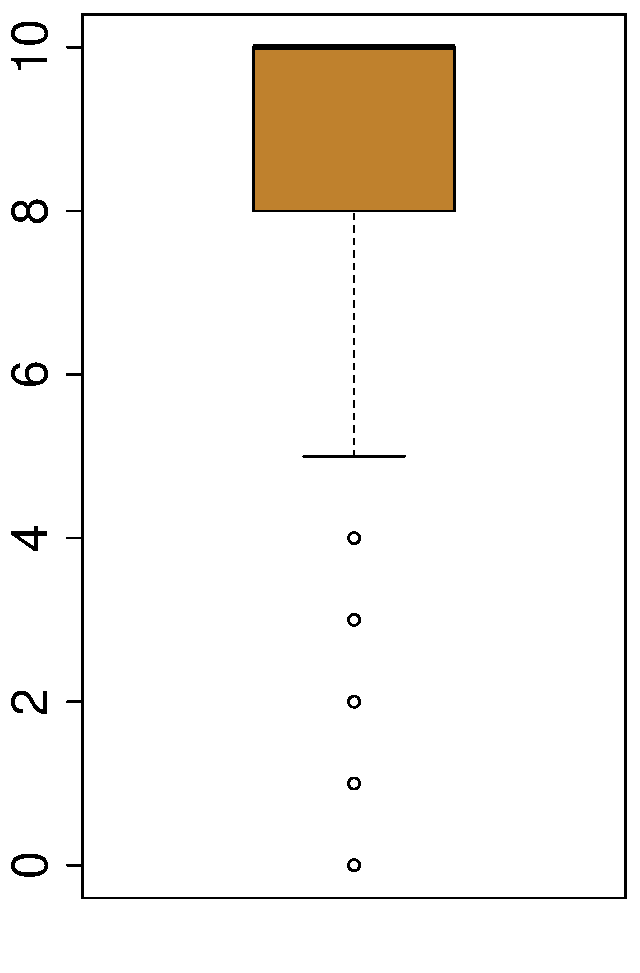
\includegraphics[width=2.7cm, height=4.0cm]{./../images/developer_experience_in_general.pdf}
		\caption{In general.}
		\label{fig:developers_experience_in_general}
	\end{subfigure} %
	\begin{subfigure}[b]{0.3\textwidth}
		\centering
		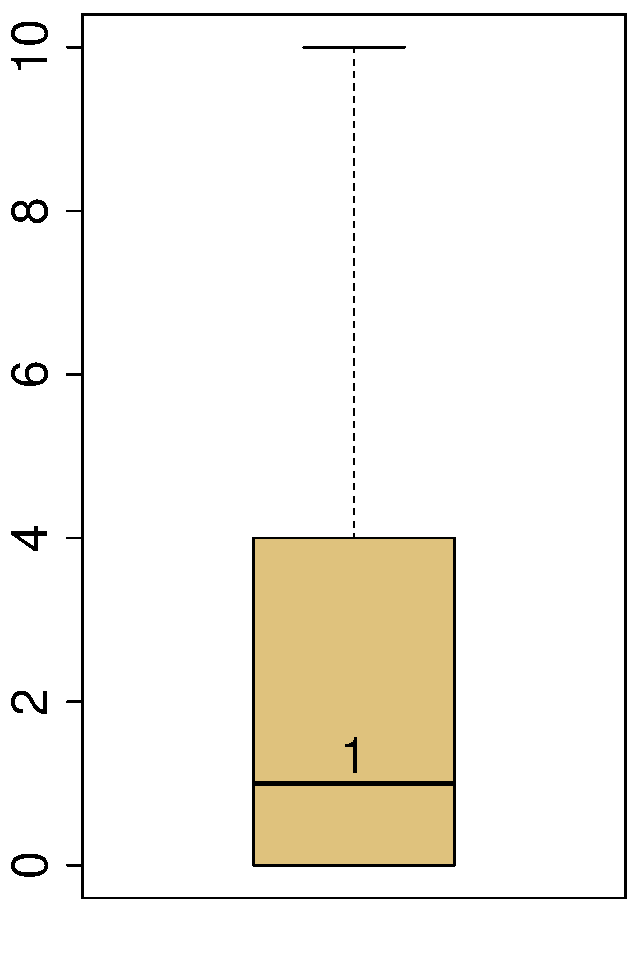
\includegraphics[width=2.5cm, height=4.0cm]{./../images/developer_experience_on_the_studied_project.pdf}
		\caption{On the studied project.}
		\label{fig:developers_experience_on_the_studied_project}
	\end{subfigure}
		\begin{subfigure}[b]{0.3\textwidth}
		\centering
		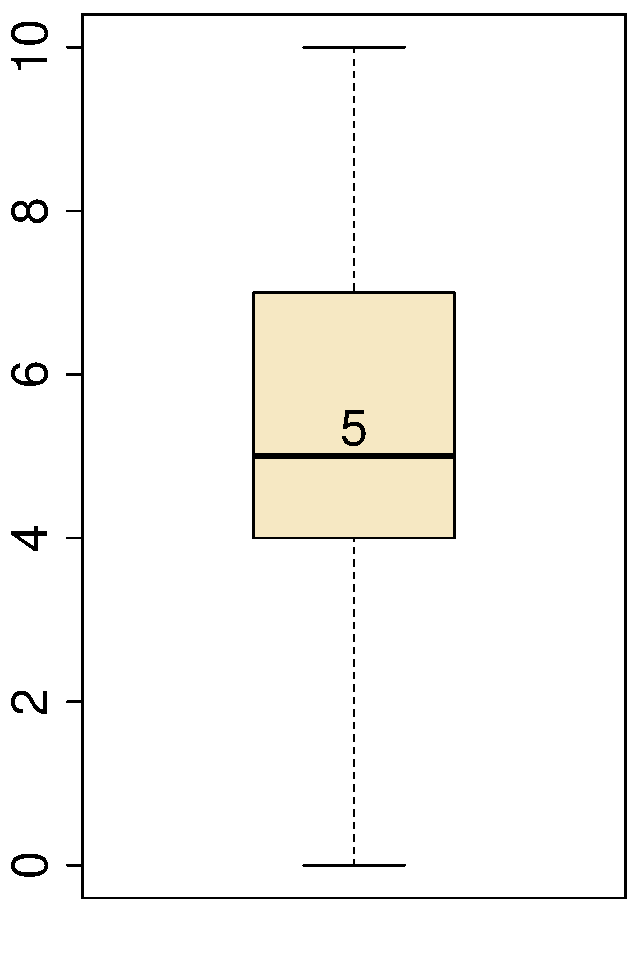
\includegraphics[width=2.5cm, height=4.0cm]{./../images/developer_experience_using_CI.pdf}  
		\caption{Using CI.}
		\label{fig:developers_experience_using_ci}
	\end{subfigure}
		\caption{Participants' experience on software developement.}
		\label{fig:developers_experience}
	\end{figure}

	Besides observing that the participants of the study are mostly experienced developers and that they also have a great familiarity contributing for projects that use continuous integration, we observe that 51.8\% (\nicefrac{226}{436}) of them have used CI in 80--100\% of the projects they worked on (see Figure \ref{fig:ratio_of_projects_using_ci}). Furthermore, we observe that  26.8\% (\nicefrac{117}{436}) the participants stated that a ration of 0--40\%  of the projects they have worked on use continuous integration. In this sense, we have different participants' profiles regarding their use of continuous integration, what could help us on identifying a general perception of the adoption of this practice on the delivery time of merged pull-requests, as well as the influence of CI on the review and releasing processes of popular open source projects.

	\begin{figure}[H]
	% Use the relevant command to insert your figure file.
	% For example, with the graphicx package use

	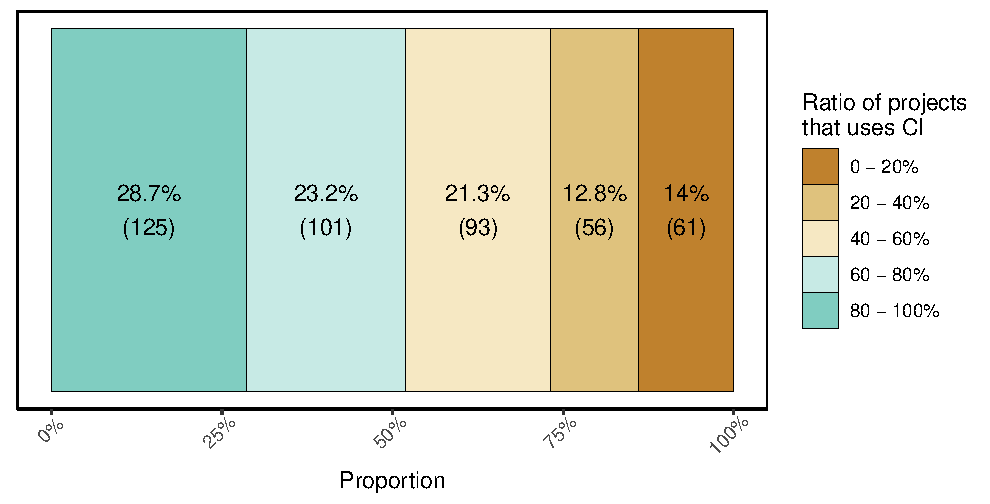
\includegraphics[height=8cm, width=11cm]{../images/ratio_of_projects_using_ci.pdf}
	% figure caption is below the figure
	\caption{Ratio of projects that the participants worked on that used continuous integration (\textit{Question \#5}).}
	\label{fig:ratio_of_projects_using_ci}       % Give a unique label
	\end{figure}

	When analyzing the participants' main activities, we observed that development is the most common activity among them, followed by test and review. A total of 92.9\% of the participants stated that development is one of the main activities on the projects they work on. Moreover, a significant 
	number of 229 (50.9\%) of the participants stated that review is also one of the main activities on their projects. Figure \ref{fig:main_development_activities} shows the participants' main activities according to their own classification (\textit{Question \#7}). Since the participant can occupy several roles, the sum of the percentages on Figure \ref{fig:main_development_activities} can be greater than 100\% once a participant is allowed to check more than one activity.

	\begin{figure}[H]
	% Use the relevant command to insert your figure file.
	% For example, with the graphicx package use
	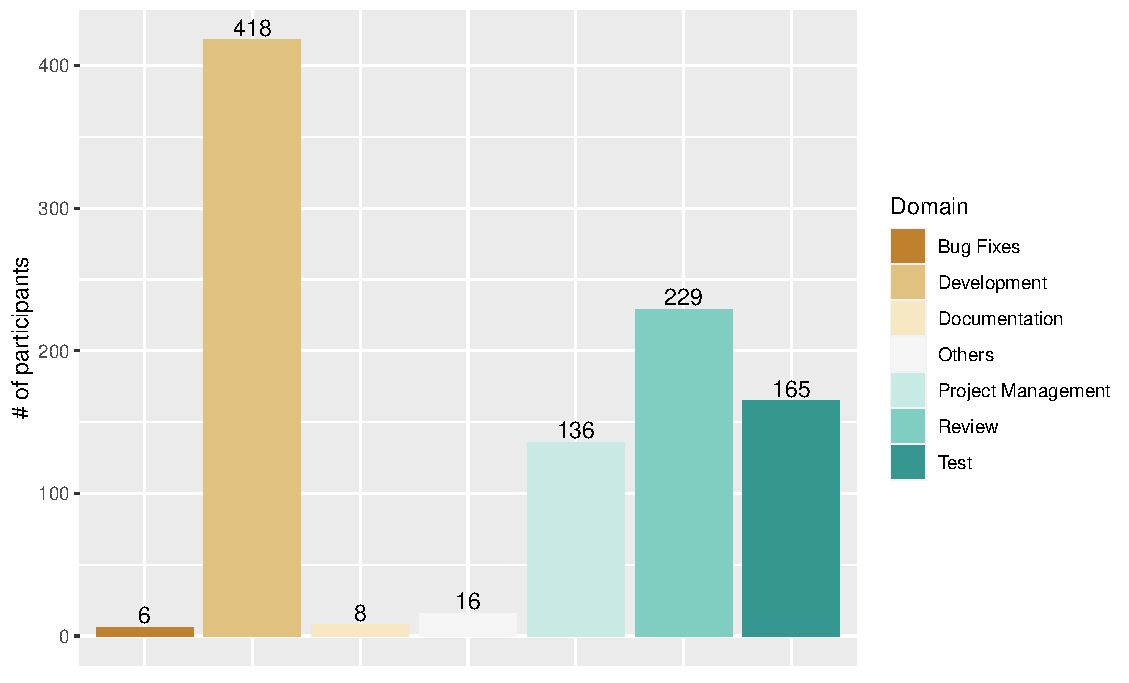
\includegraphics[height=8cm, width=12cm]{../images/main_development_activities.pdf}
	% figure caption is below the figure
	\caption{Participants' main activities.}
	\label{fig:main_development_activities}       % Give a unique label
	\end{figure}

	Furthermore, we observe that web development is the most common domain area of the participants of our study. 77.8\% (\nicefrac{350}{450}) of the participants stated that web development is one of their main domain areas (\textit{Question \#8}). The second and third most common area among them are business development (35.3\%, \nicefrac{159}{450}) and mobile application (32.2\%, \nicefrac{145}{450}), respectively. A significant number of participants are from areas such as scientific development and big data as well, which shows that our study is able to get insights from participants with several roles and development areas.

	\begin{figure}[H]
	% Use the relevant command to insert your figure file.
	% For example, with the graphicx package use
	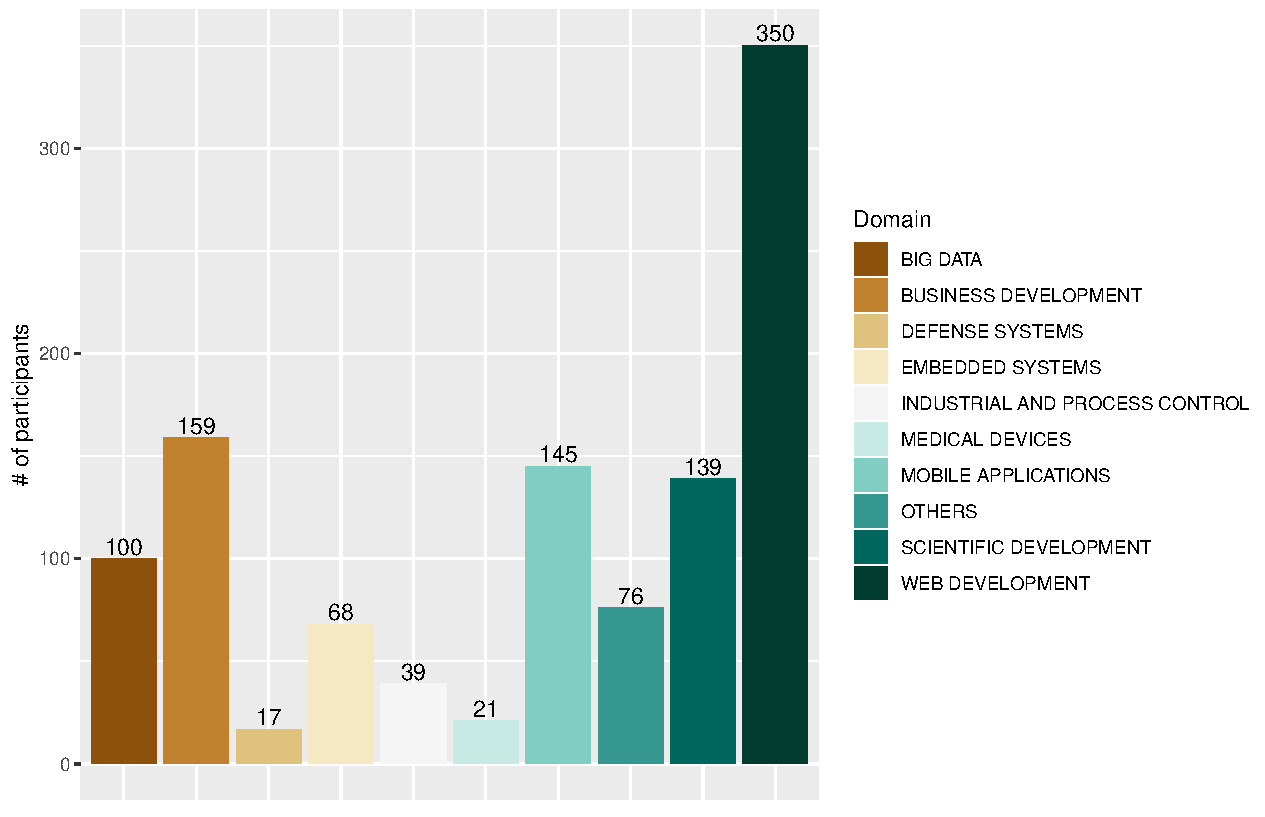
\includegraphics[height=8cm, width=12cm]{../images/developer_domain_area.pdf}
	% figure caption is below the figure
	\caption{Participants' domain area.}
	\label{fig:developer_domain_area}       % Give a unique label
	\end{figure}

	Finally, we observe that most part (77\%, \nicefrac{338}{441}) of the participants agree with the statement that continuous integration impacts the delivery time of merged pull-requests. Moreover, 16\% (\nicefrac{72}{441}) participants are neutral when asked about their perception of the impact of CI on the delivery time of pull-requests, while 7\% (\nicefrac{31}{441}) do not think continuous integration can have any impact on this (see Figure \ref{fig:developer_perception_about_impact_of_ci_on_delivery_time}).
	
	\begin{figure}[H]
		% Use the relevant command to insert your figure file.
		% For example, with the graphicx package use
		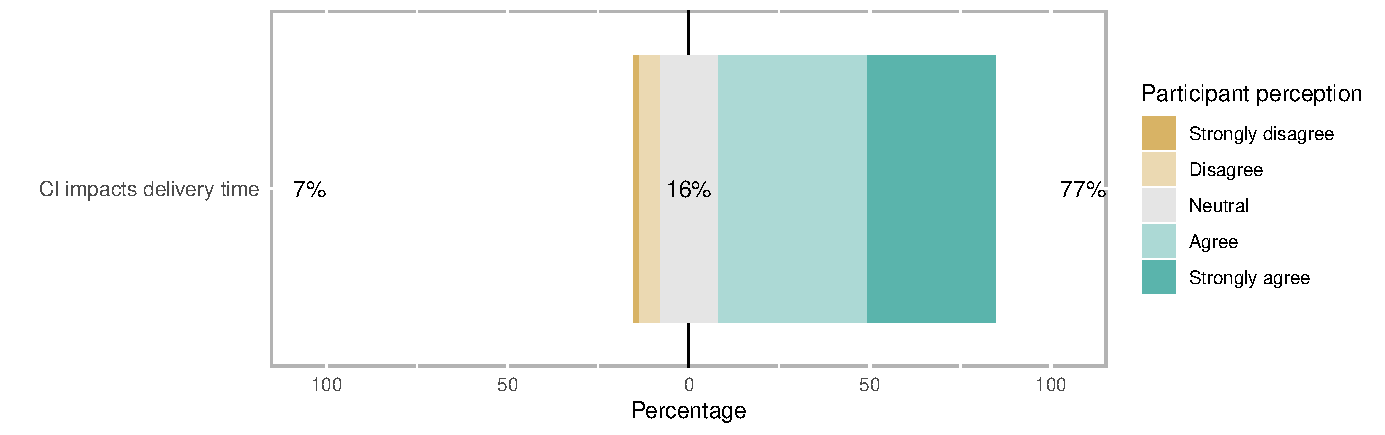
\includegraphics[height=4cm, width=12cm]{../images/developers_accordance_on_the_impact_of_ci_on_delivery_time.pdf}
		% figure caption is below the figure
		\caption{Developer's perception about the impact of continuous integration on the delivery time of merged pull-requests (\textit{Question \#12}).}
		\label{fig:developer_perception_about_impact_of_ci_on_delivery_time}       % Give a unique label
	\end{figure}



	% Table generated by Excel2LaTeX from sheet 'sheet1'
\begin{table}[htbp]
  \centering
  \caption{Add caption}
    \begin{tabular}{lc}
    \toprule
    \textbf{Metric} & \textbf{Mean} \\
    \midrule
    The contributor experience & 4.0 \\
    The time at which a pull request is merged during a release cycle & 3.7 \\
    The time that previously submitted PRs of a contributor were delivered & 3.6 \\
    The description size of a PR & 3.5 \\
    A PR has a stacktrace attached & 3.4 \\
    The number of PRs waiting to be delivered at the moment that a new PR was merged & 2.9 \\
    The number of files attached to a PR & 2.8 \\
    The number of comments recorded on a PR & 2.7 \\
    Number of commits in a PR & 2.7 \\
    The time interval between the PR comments & 2.7 \\
    The time that a pull request waited to be merged & 2.7 \\
    Number of lines of code in a PR & 2.4 \\
    \bottomrule
    \end{tabular}%
  \label{tab:addlabel}%
\end{table}%

	
	%\paragraph{Paragraph headings} Use paragraph headings as needed.
	%\begin{equation}
	%a^2+b^2=c^2
	%\end{equation}
	%
	%% For one-column wide figures use
	%\begin{figure}
	%% Use the relevant command to insert your figure file.
	%% For example, with the graphicx package use
	%  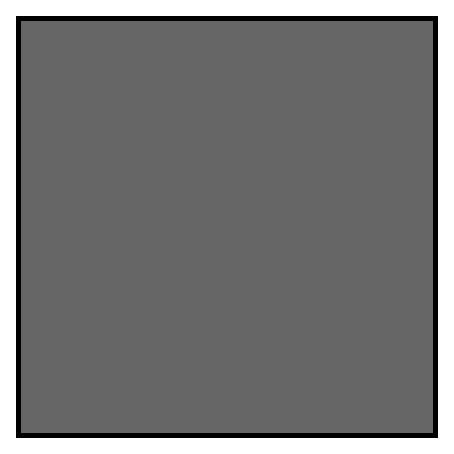
\includegraphics{example.eps}
	%% figure caption is below the figure
	%\caption{Please write your figure caption here}
	%\label{fig:1}       % Give a unique label
	%\end{figure}
	%%
	%% For two-column wide figures use
	%\begin{figure*}
	%% Use the relevant command to insert your figure file.
	%% For example, with the graphicx package use
	%  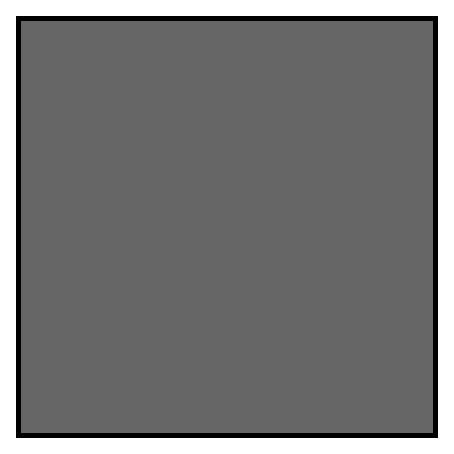
\includegraphics[width=0.75\textwidth]{example.eps}
	%% figure caption is below the figure
	%\caption{Please write your figure caption here}
	%\label{fig:2}       % Give a unique label
	%\end{figure*}
	%%
	%% For tables use
	%\begin{table}
	%% table caption is above the table
	%\caption{Please write your table caption here}
	%\label{tab:1}       % Give a unique label
	%% For LaTeX tables use
	%\begin{tabular}{lll}
	%\hline\noalign{\smallskip}
	%first & second & third  \\
	%\noalign{\smallskip}\hline\noalign{\smallskip}
	%number & number & number \\
	%number & number & number \\
	%\noalign{\smallskip}\hline
	%\end{tabular}
	%\end{table}
	
	
	%\begin{acknowledgements}
	%If you'd like to thank anyone, place your comments here
	%and remove the percent signs.
	%\end{acknowledgements}
	
	
	% Authors must disclose all relationships or interests that 
	% could have direct or potential influence or impart bias on 
	% the work: 
	%
	% \section*{Conflict of interest}
	%
	% The authors declare that they have no conflict of interest.
	
	
	% Appendix starts here
	\newpage
	\appendix
	
	\section*{Appendix A: Project Survey Example}
	\label{sec:appendix_project_survey_example}
	
	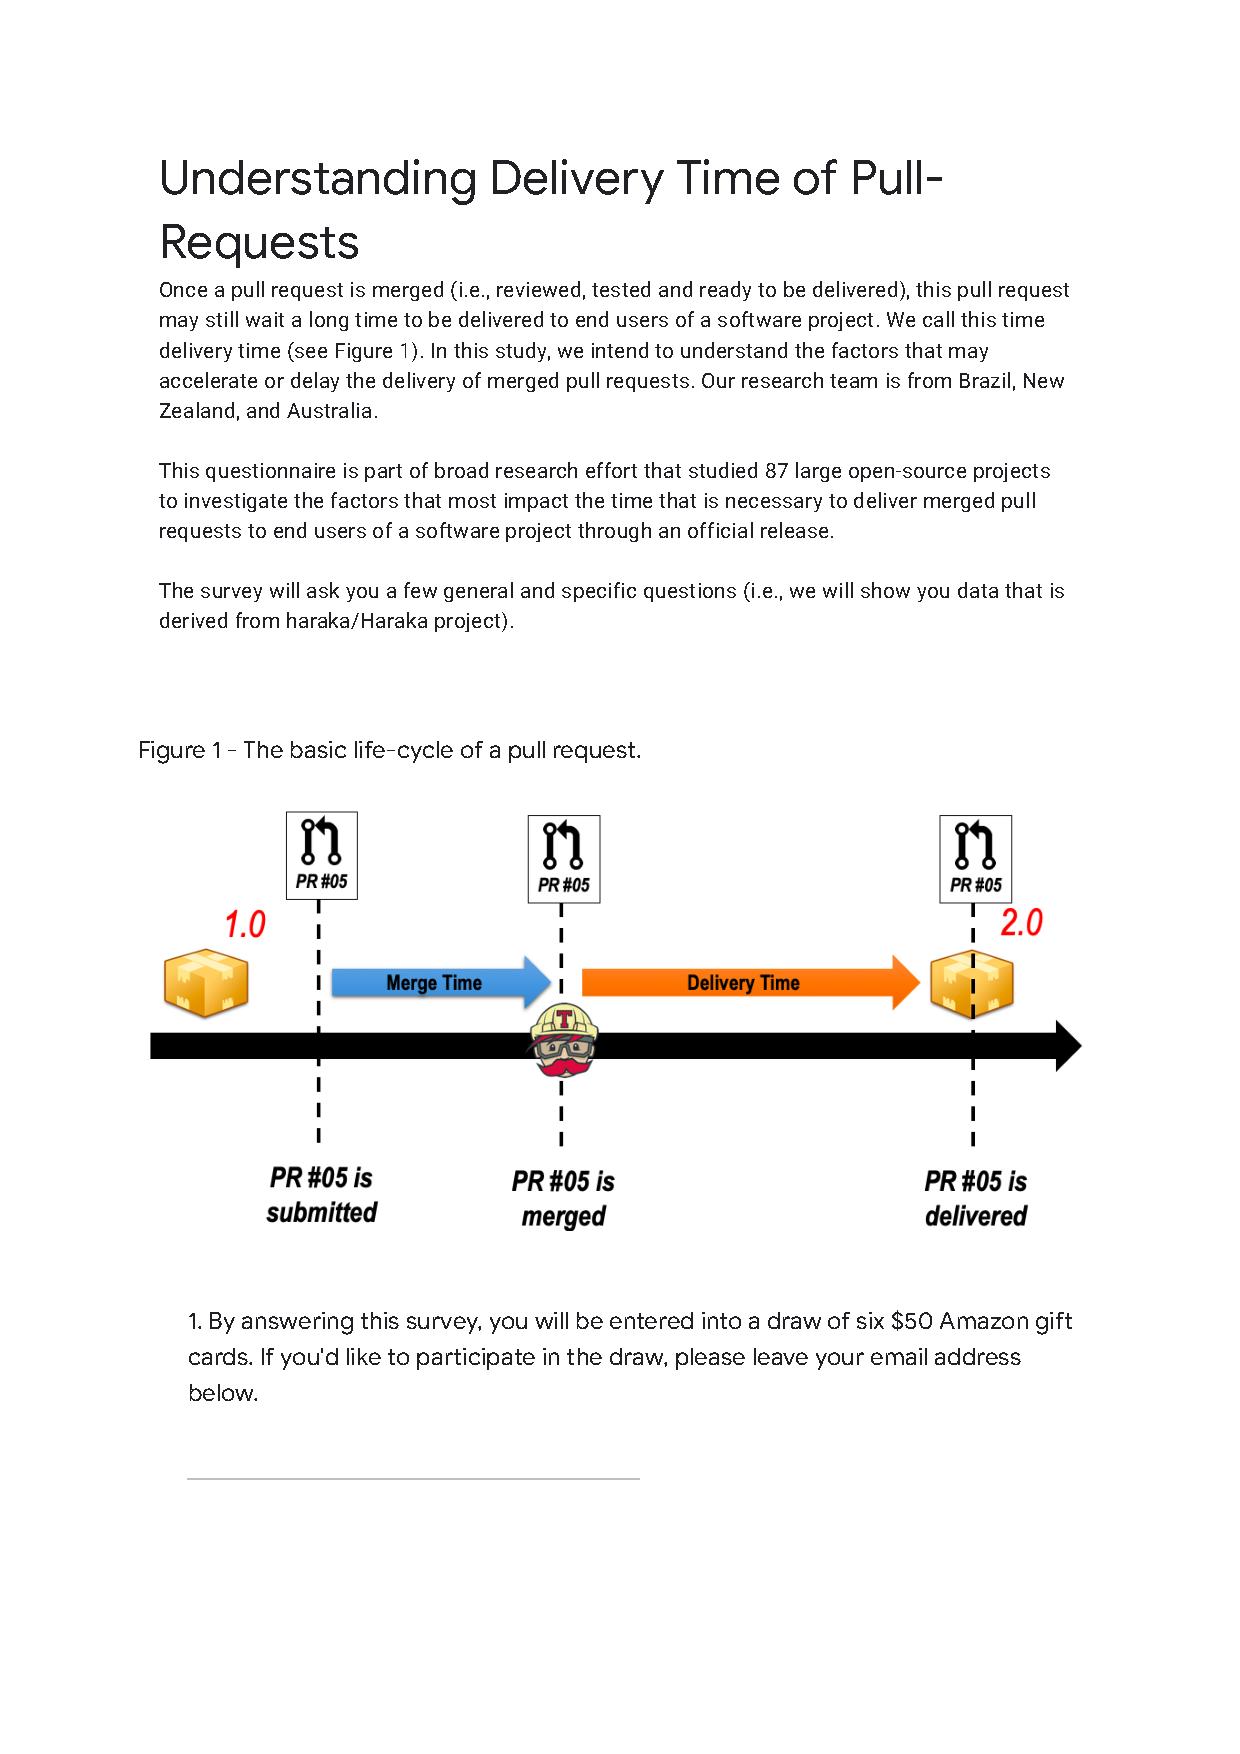
\includepdf[pages=-]{haraka_Haraka_form.pdf}
	
	\section*{Appendix A: Invitation Letter}
	\label{sec:appendix_invitation_latter}
	
	MAIL SUBJECT: Why do PRs take so long to be delivered? Research survey
	
	Dear \${contributor.name},
	
	We are a group of researchers from universities based in Brazil, Australia, and New Zealand. We are studying the impact of Continuous Integration on the time to release merged pull requests to end users of open source projects.
	
	We have collected public data from the project \${project.fullName} in the period from \${project.creationDate} to 2016-11-11. According to our data, you have contributed \${contributor.deliveredPRsCount} pull-requests to \${project.fullName} which were effectively merged and delivered to end users. 
	
	As you were a contributor of the project \${project.fullName}, we would appreciate if you shared your experience with us by answering a few questions in the following survey: 
	
	Google Form: Understanding Delivery Time of Pull Requests
	
	The survey has 24 questions (all of them are optional) and will take less than 15 minutes to complete. To compensate you for your time, all participants that answer all questions will be entered into a draw of six \$50 Amazon gift cards.
	
	Best Regards,
	João Helis Bernardo.
	PhD student at the Federal University of Rio Grande do Norte, Brazil.
	
	
	% BibTeX users please use one of
	\bibliographystyle{spbasic}      % basic style, author-year citations
	%\bibliographystyle{spmpsci}      % mathematics and physical sciences
	%\bibliographystyle{spphys}       % APS-like style for physics
	%\bibliography{}   % name your BibTeX data base
	
	% Non-BibTeX users please use
	
	\bibliography{references}
	
	%\begin{thebibliography}{}
	%%
	%% and use \bibitem to create references. Consult the Instructions
	%% for authors for reference list style.
	%%
	%\bibitem{RefJ}
	%% Format for Journal Reference
	%Author, Article title, Journal, Volume, page numbers (year)
	%% Format for books
	%\bibitem{RefB}
	%Author, Book title, page numbers. Publisher, place (year)
	%% etc
	%\end{thebibliography}
	
\end{document}
% end of file template.tex